\documentclass[border=10pt]{standalone}

\usepackage{tikz}
\usepackage{tikzsymbols}
\usetikzlibrary{calc,patterns,shapes.geometric}

\def\centerarc[#1](#2)(#3:#4:#5){\draw[#1] ($(#2)+({#5*cos(#3)},{#5*sin(#3)})$) arc (#3:#4:#5);}

\begin{document}
	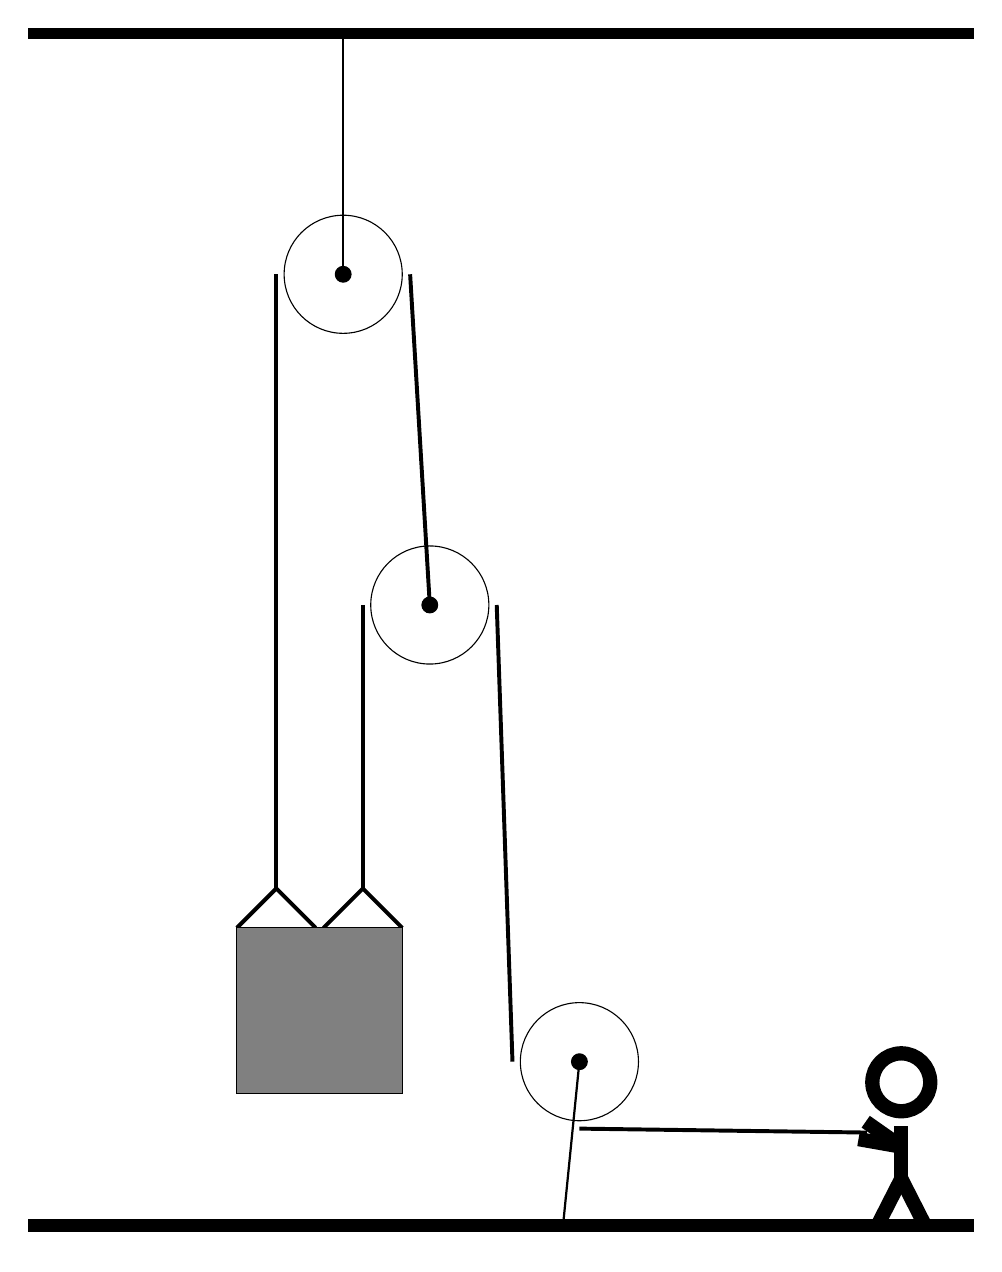
\begin{tikzpicture}
		%%%%% START %%%%%
		\draw[fill=black] (-2, 12) rectangle (10, 12.125);
		
		\draw (2, 9.0) circle (0.75);
		\draw[fill=black] (2, 9.0) circle (0.1);
		\draw[thick] (2, 9.0) -- (2, 12);
		
		\draw (3.1, 4.8) circle (0.75);
		\draw[fill=black] (3.1, 4.8) circle (0.1);
		
		\draw (5, -1) circle (0.75);
		\draw[fill=black] (5, -1) circle (0.1);
		\draw[thick] (5, -1) -- (4.8, -3);
		
		\draw[line width = 0.5mm]  (0.65, 0.7) -- (1.15, 1.2) -- (1.65, 0.7);
		\draw[line width = 0.5mm]  (1.75, 0.7) -- (2.25, 1.2) -- (2.75, 0.7);
		\draw[fill=black!50] (0.65, 0.7) rectangle (2.75, -1.4);
		
		\draw[line width = 0.5mm] (1.15, 9.0) -- (1.15, 1.2);
		\centerarc[line width = 0.5mm](2, 9.0)(0:180:0.85);
		\draw[line width = 0.5mm] (2.85, 9.0) -- (3.1, 4.8);
		\draw[line width = 0.5mm] (2.25, 4.8) -- (2.25, 1.2);
		\centerarc[line width = 0.5mm](3.1, 4.8)(0:180:0.85);
		\draw[line width = 0.5mm] (3.95, 4.8) -- (4.15, -1);
		\centerarc[line width = 0.5mm](5, -1)(180:270:0.85);
		\draw[line width = 0.5mm] (5, -1.85) -- (8.65, -1.9);
		
		\node at (9, -2) {\Strichmaxerl[10][-35][170]};
		
		\draw[fill=black] (-2, -3) rectangle (10, -3.15);
		%%%%% END %%%%%
	\end{tikzpicture}
\end{document}